\autsection{Front End Mockups}{Daniel Santiago}
\label{sec:mockups}

This section contains mockups that the team developed to design Panda Code Reviews front end along with an explanation of the expected behavior. Note that this is part of the design of the project and does not necessarily reflects the final view of the site.

\textbf{Site Home Page:} The site homepage includes information and
marketing information about Panda Code Reviews and the services that it offers.
It also includes links for logging in and signing up. If the user is already
logged in, it also includes links for accessing his account home page and
general account settings.

\begin{figure}[H]
	\centering
	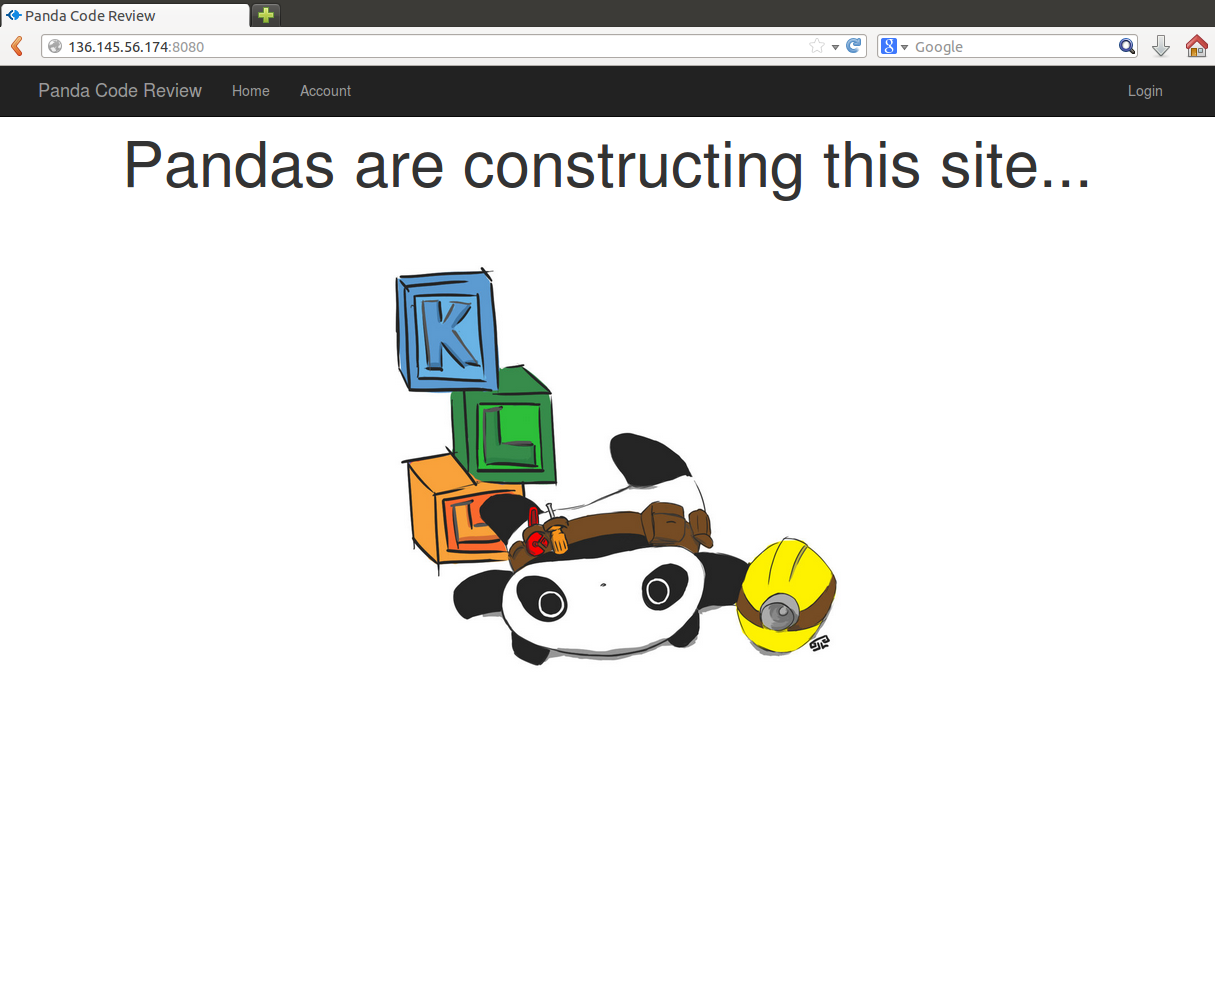
\includegraphics[width=\textwidth]{img/index}
	\caption{Site Home Page}
\end{figure}

\textbf{Login and Sign Up:} The login screen and sign up screen asks for
the users e-mail and password. If the user clicks the sign up button, it asks
for the necessary information to create and account: name,
email, password and school.

\begin{figure}[H]
	\centering
	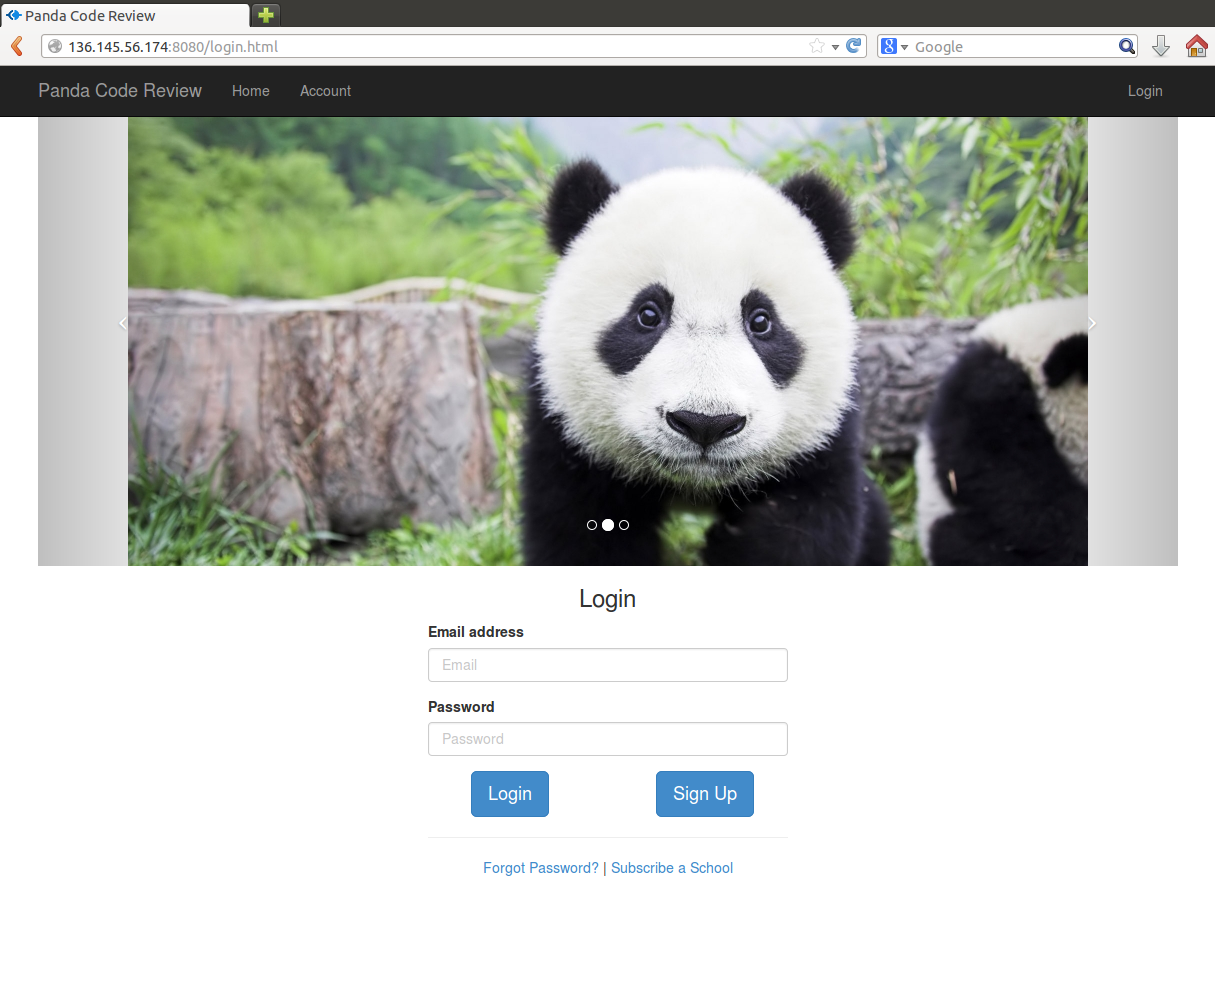
\includegraphics[width=\textwidth]{img/login}
	\caption{Login}
\end{figure}

\begin{figure}[H]
	\centering
	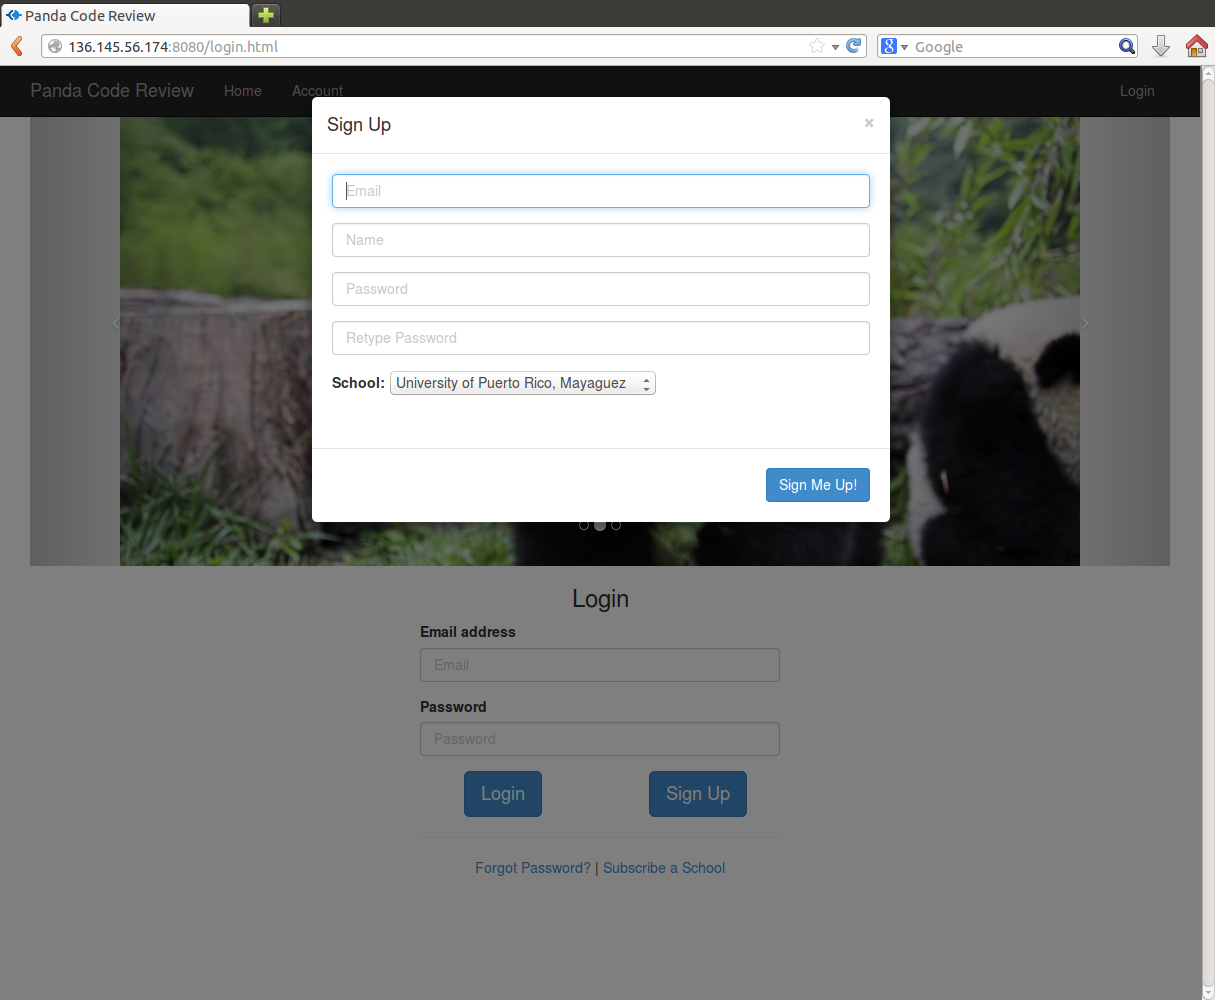
\includegraphics[width=\textwidth]{img/signup}
	\caption{Sign Up}
\end{figure}

\textbf{Account Home:} The account home shows different things
depending on the user. If the user is a student, the account home shows the
enrolled courses and also contains a button for enrolling new courses. Each
course contains a snippet of the assignments that are due and the dates
at which they are due. The student can click on the course name to see more
information about the course, and he can also click on the due assignment
names to see more information about the assignments. In the case of a professor,
he can see the list of courses, and can also create a new course.
The professor is also able to see the amount of students enrolled in the
course and the names, contact emails, and summary of grades of each student.

\begin{figure}[H]
	\centering
	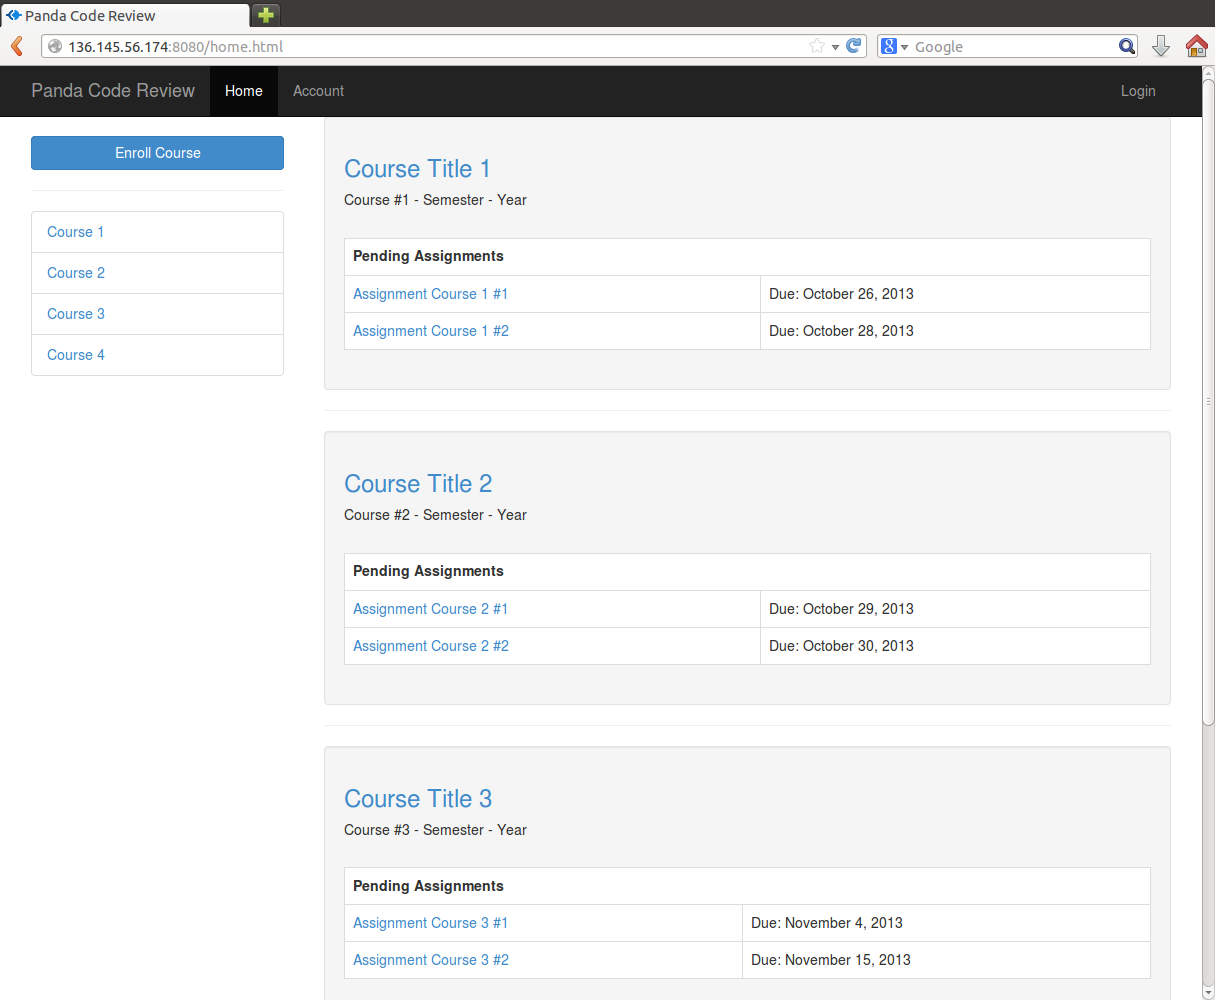
\includegraphics[width=\textwidth]{img/courses}
	\caption{Account Home - Student}
\end{figure}

\begin{figure}[H]
	\centering
	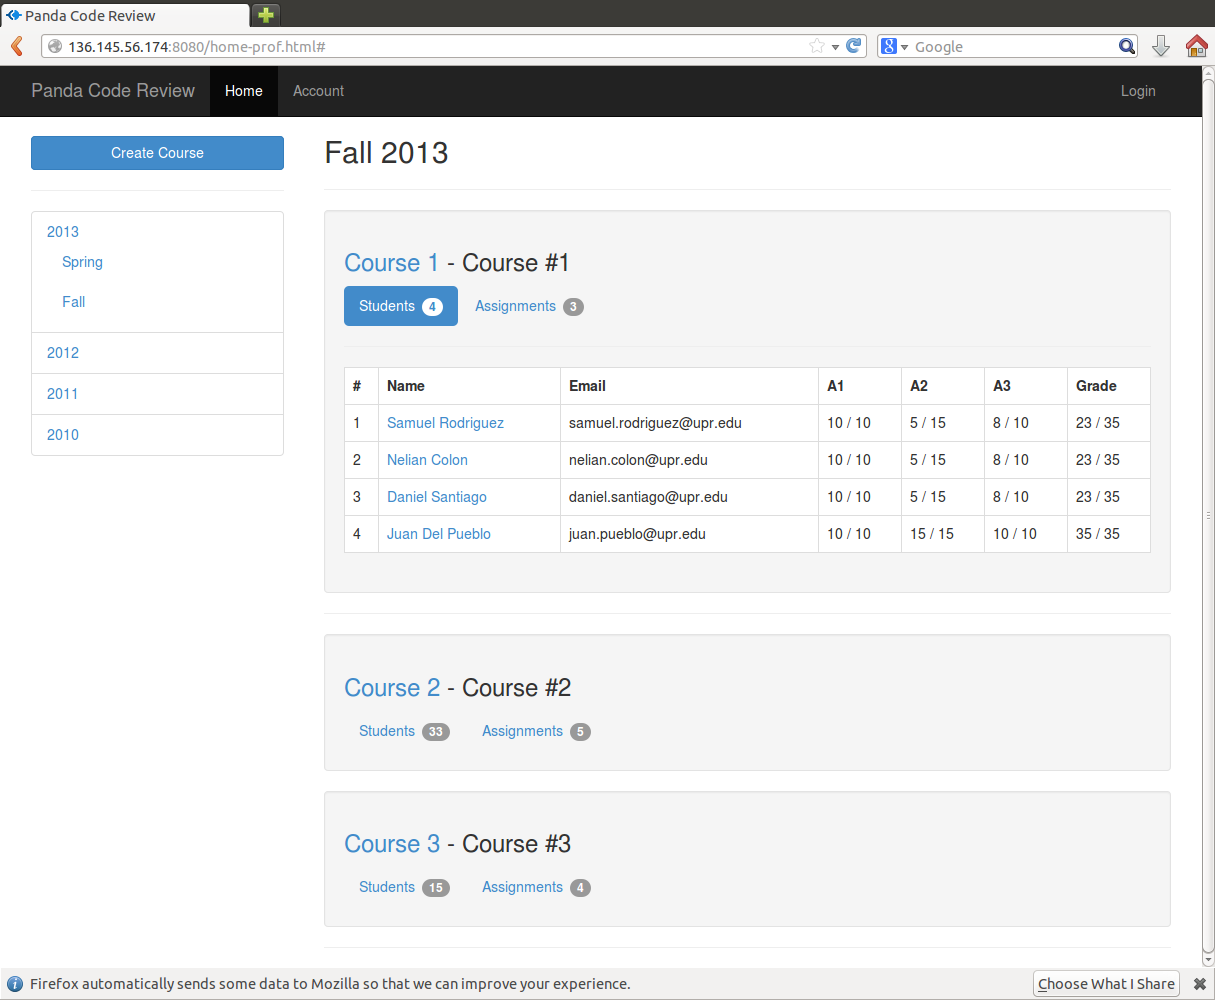
\includegraphics[width=\textwidth]{img/courses-prof}
	\caption{Account Home - Professor}
\end{figure}

\textbf{Create Course:} The professor is the only one that can see the
create course view. This view is included as part of the account home of the
professor, it is a drop down that asks for the new course's information. After
creating the course, the professor can edit it and add students.

\textbf{View Course:} Students and professors can view detail information
about a course. In case of the student, he can to see basic information
about the course, like course title, number, semester, and year. He can also see
a summary of his grade, his assignments, and his submissions. He can also see
contact information of his professor in a glance. A professor can see with great
detail the amount of students in the course, and the assignments that he
currently has in the course. He can also edit and delete the course from this
view, and can create new assignments to add to the course.

\begin{figure}[H]
	\centering
	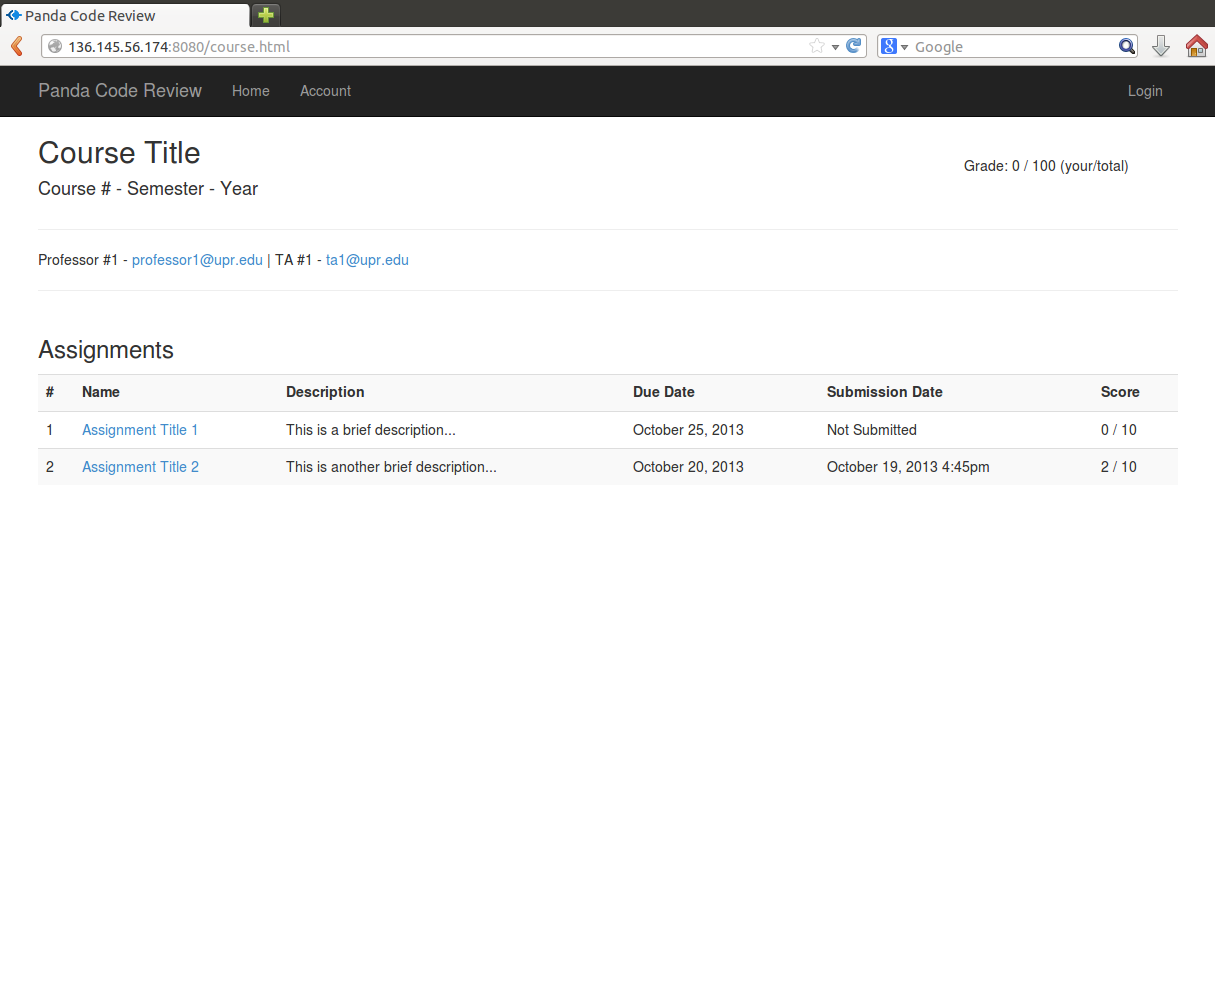
\includegraphics[width=\textwidth]{img/course}
	\caption{View Course - Student}
\end{figure}

\begin{figure}[H]
	\centering
	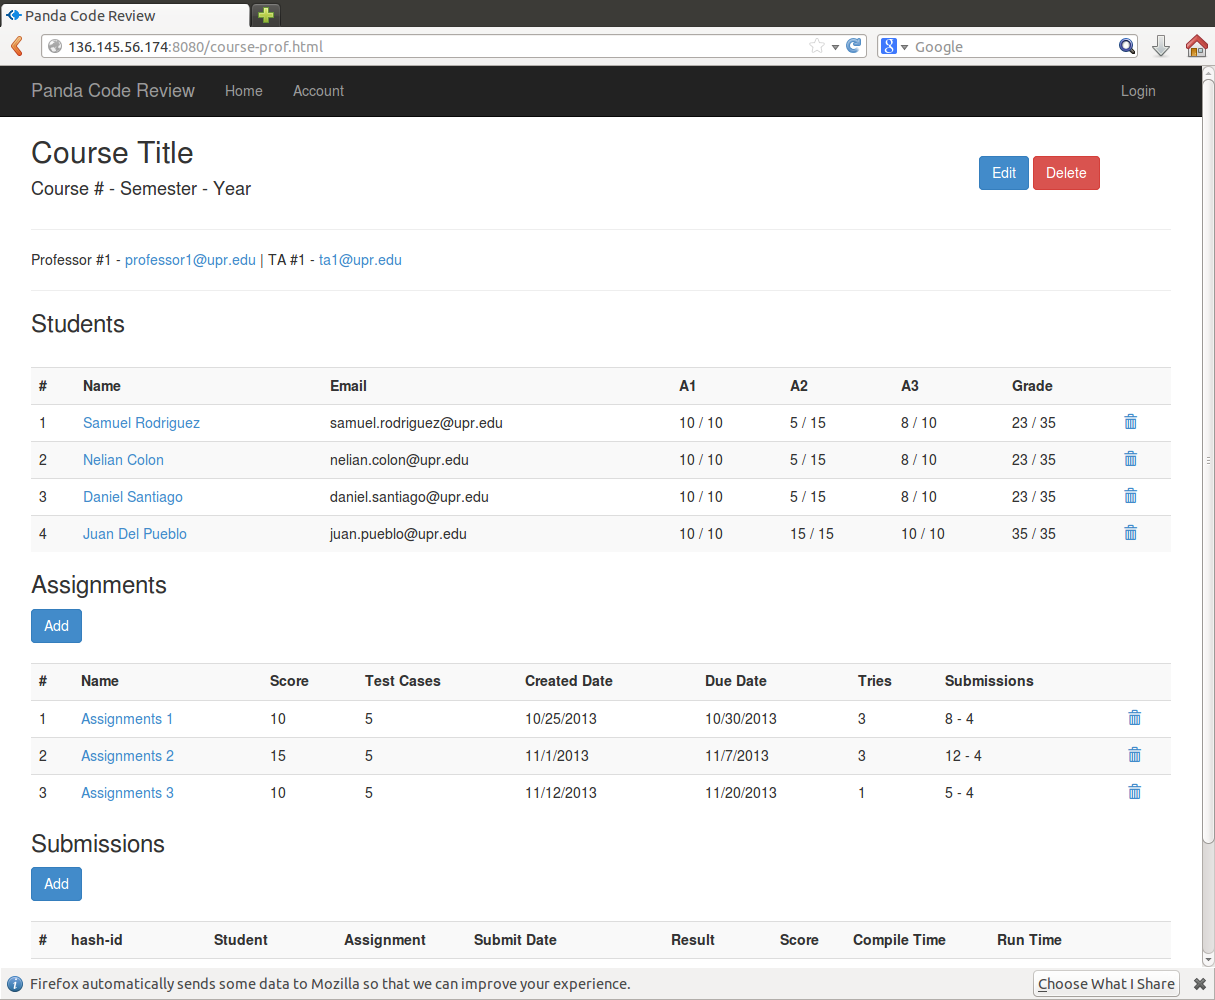
\includegraphics[width=\textwidth]{img/course-prof}
	\caption{View Course - Professor}
\end{figure}

\textbf{Enroll Course:} The student can easily enroll in a course in the
enroll course view which is part of the student's account home view. This view
is a drop down that only asks for the courses name. This is a searching feature.
As the student types up the name, it instantly provides results. The student
can then select a course and enroll in it.

\textbf{Create Assignment:} The professor can create an assignment in his
course view. This view is a drop down, where the professor can add the name and
the due date of the assignment. Once the assignment has been created the
professor can add test cases to it.

\textbf{Assignment Information:} Professors and students can see this
view. For the students, the information view contains the description, the
instructions for completing the assignment, the due date, the student's score,
and the last submission date. The professor also has the ability to view the
scores of every student, and can also edit and delete information from the
assignment. A student can only view the information of the assignment and can
only view his own grade.

\begin{figure}[H]
	\centering
	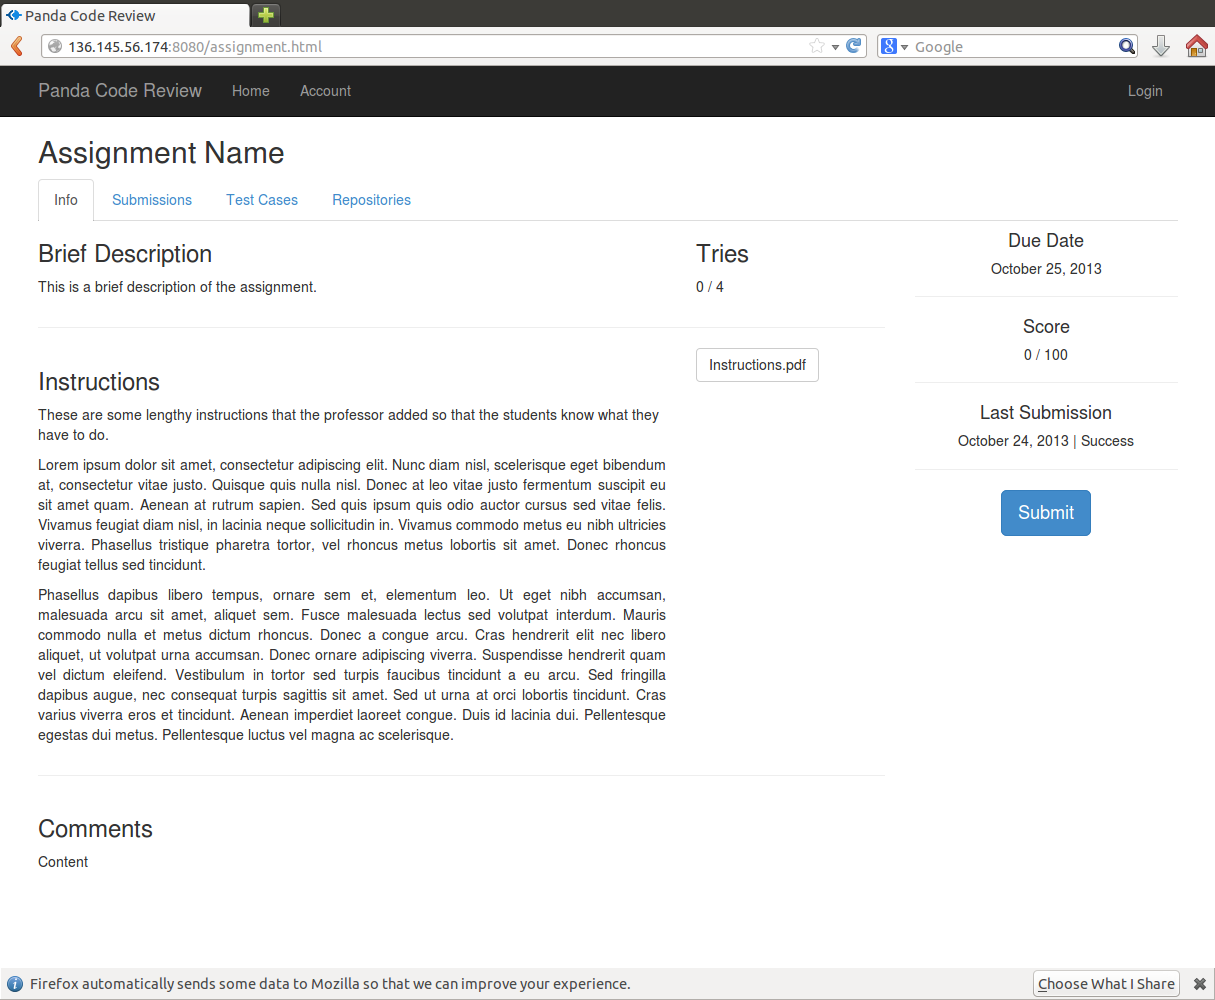
\includegraphics[width=\textwidth]{img/assignment-info}
	\caption{Assignment Information - Student}
\end{figure}

\begin{figure}[H]
	\centering
	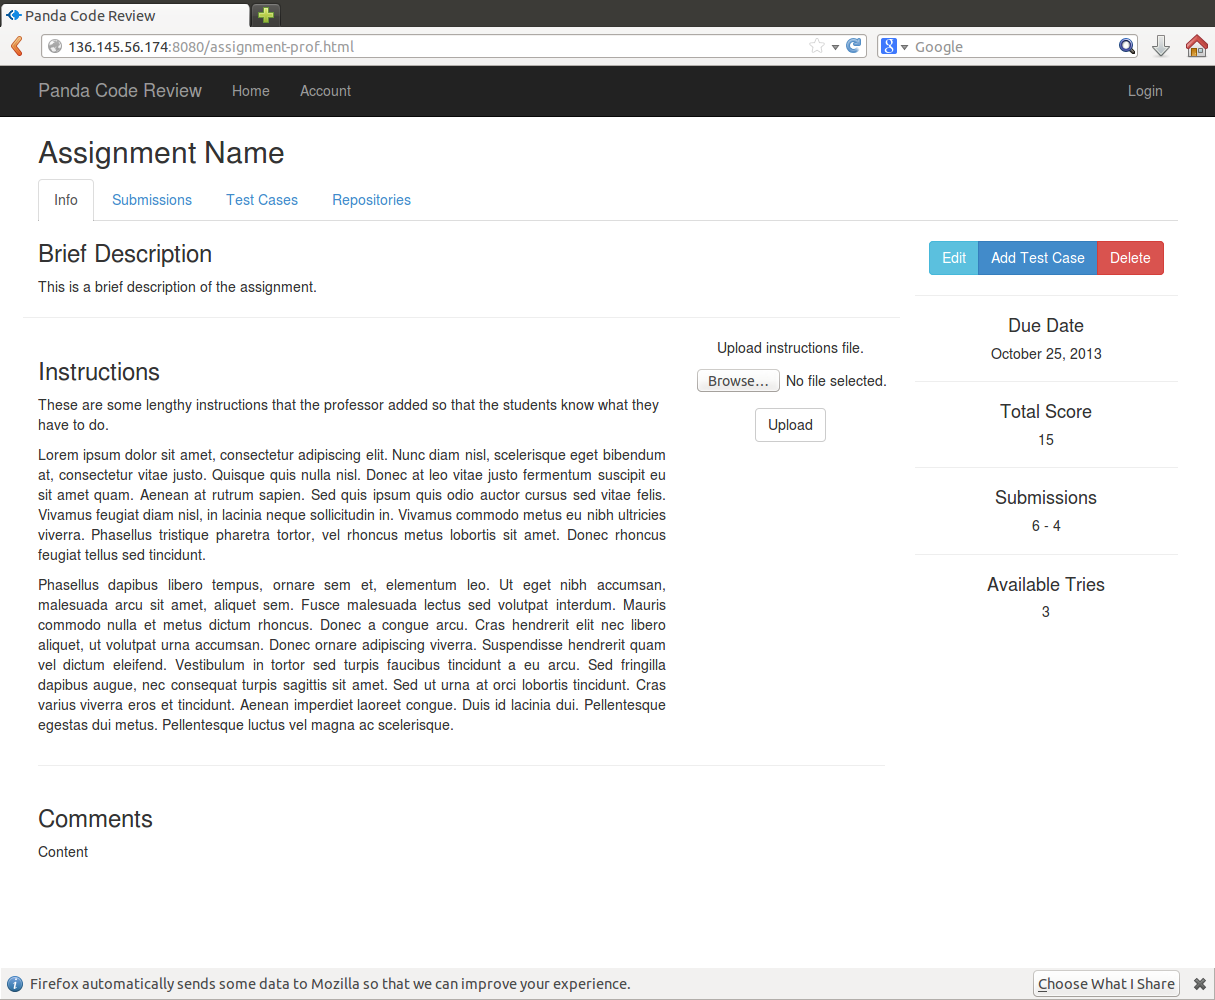
\includegraphics[width=\textwidth]{img/assignment-info-prof}
	\caption{Assignment Information - Professor}
\end{figure}

\textbf{Assignment Submissions:} Both students and professors can see the
assignment submissions. The difference is that the students can only see their
own submissions, whereas the professor can see the submissions of every single
student. The submission information includes the hash id, the student's
name, the submit date, the result of the submission, the score, the compile time
of the submission, and the run time of the submission. The professor also
has an additional button that allows him to override the grade of a student.

\begin{figure}[H]
	\centering
	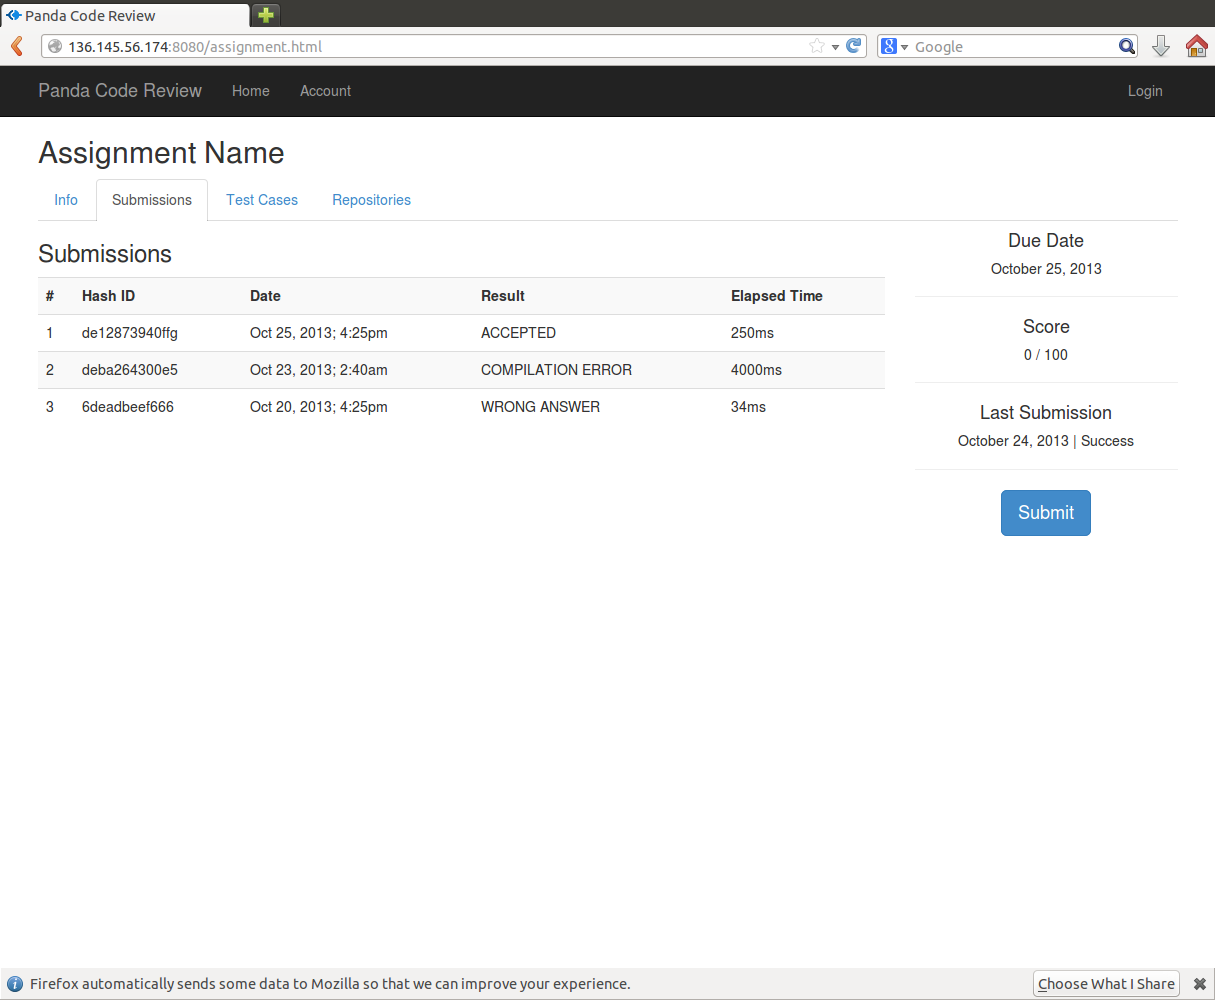
\includegraphics[width=\textwidth]{img/assignment-sub}
	\caption{Assignment Submissions - Student}
\end{figure}

\begin{figure}[H]
	\centering
	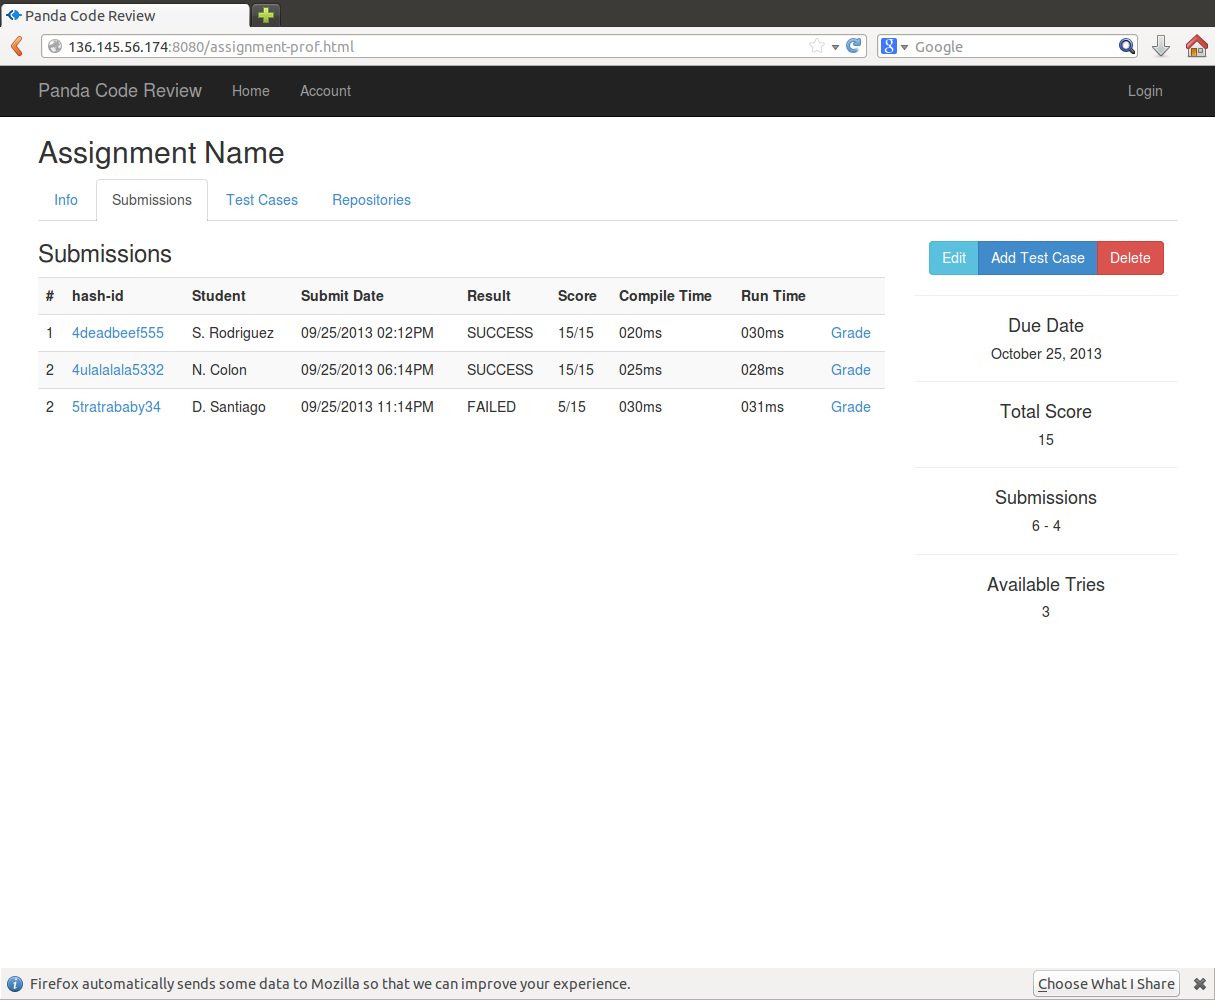
\includegraphics[width=\textwidth]{img/assignment-sub-prof}
	\caption{Assignment Submissions - Professor}
\end{figure}

\textbf{Assignment Repositories:} Both the students and the professors can
see the repositories, but the student can only see his own repositories whereas
the professors can see the repositories of every student.

\begin{figure}[H]
	\centering
	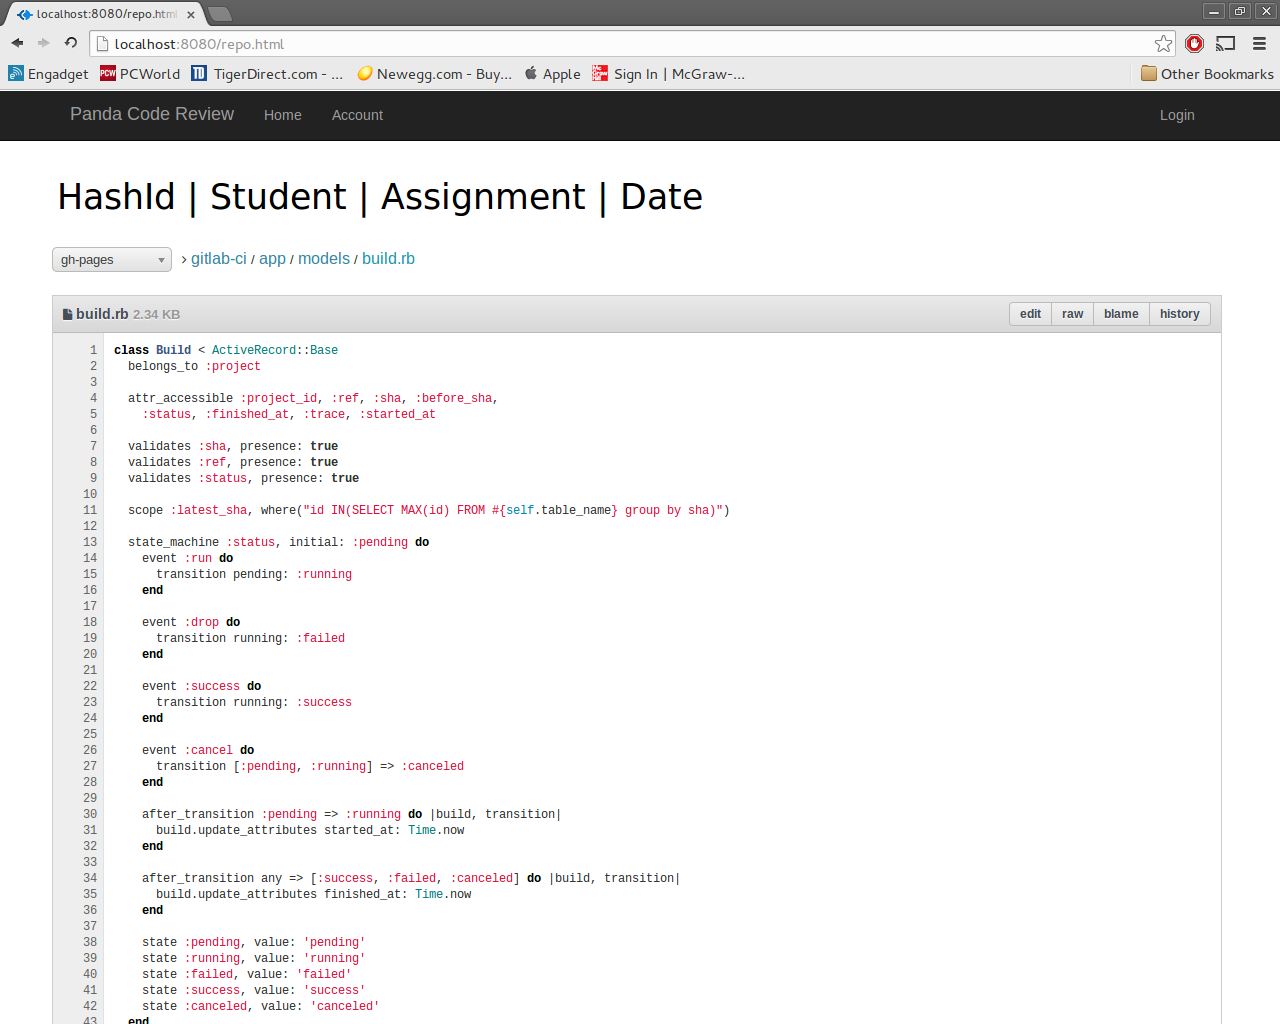
\includegraphics[width=\textwidth]{img/repo}
	\caption{Git Repository}
\end{figure}

\textbf{Assignment Test Cases:} Both students and professors can see the
assignment test cases, the difference is that the professor can add, edit and
delete test cases, whereas the student can only view them and develop his
assignment accordingly.

\begin{figure}[H]
	\centering
	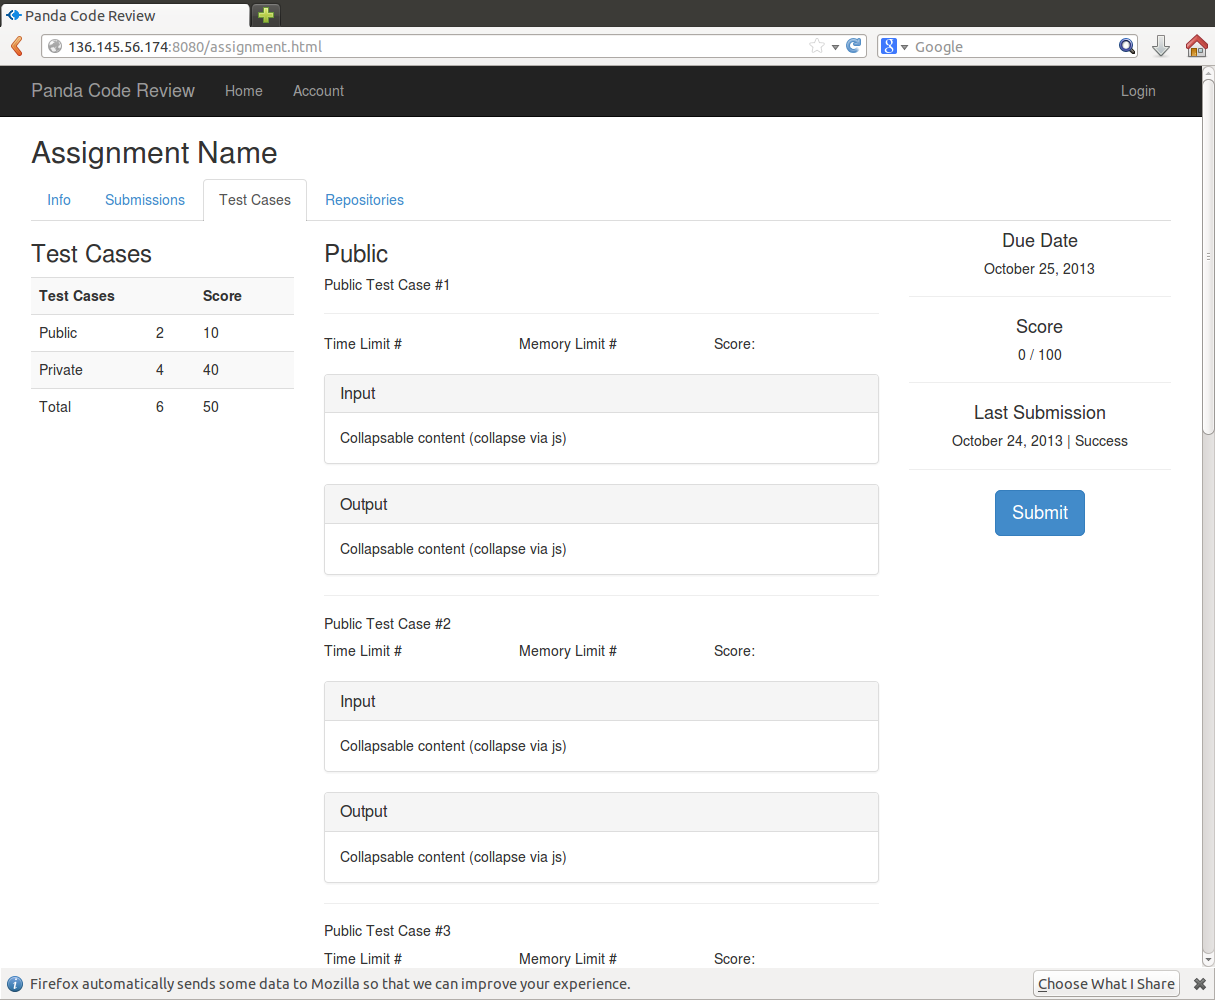
\includegraphics[width=\textwidth]{img/assignment-test}
	\caption{Assignment Test Cases}
\end{figure}

\textbf{Add test cases:} The professor can add test cases in the
assignment test cases view. This asks for the input of the test case and the
expected output. Optionally the professor can also set time and memory limits.

\textbf{Grade:} Both students and professor can see grades. The students
can see their own grade from the assignment view and from the course view. The
student can view grades from specific assignments or total grades for
specific courses. The professors can see the grades of every student for his
courses and assignments. He can also modify their grades.

\textbf{Account Profile:} Both students and professors can see
their respective account profiles. They can also edit it accordingly.


\begin{figure}[H]
	\centering
	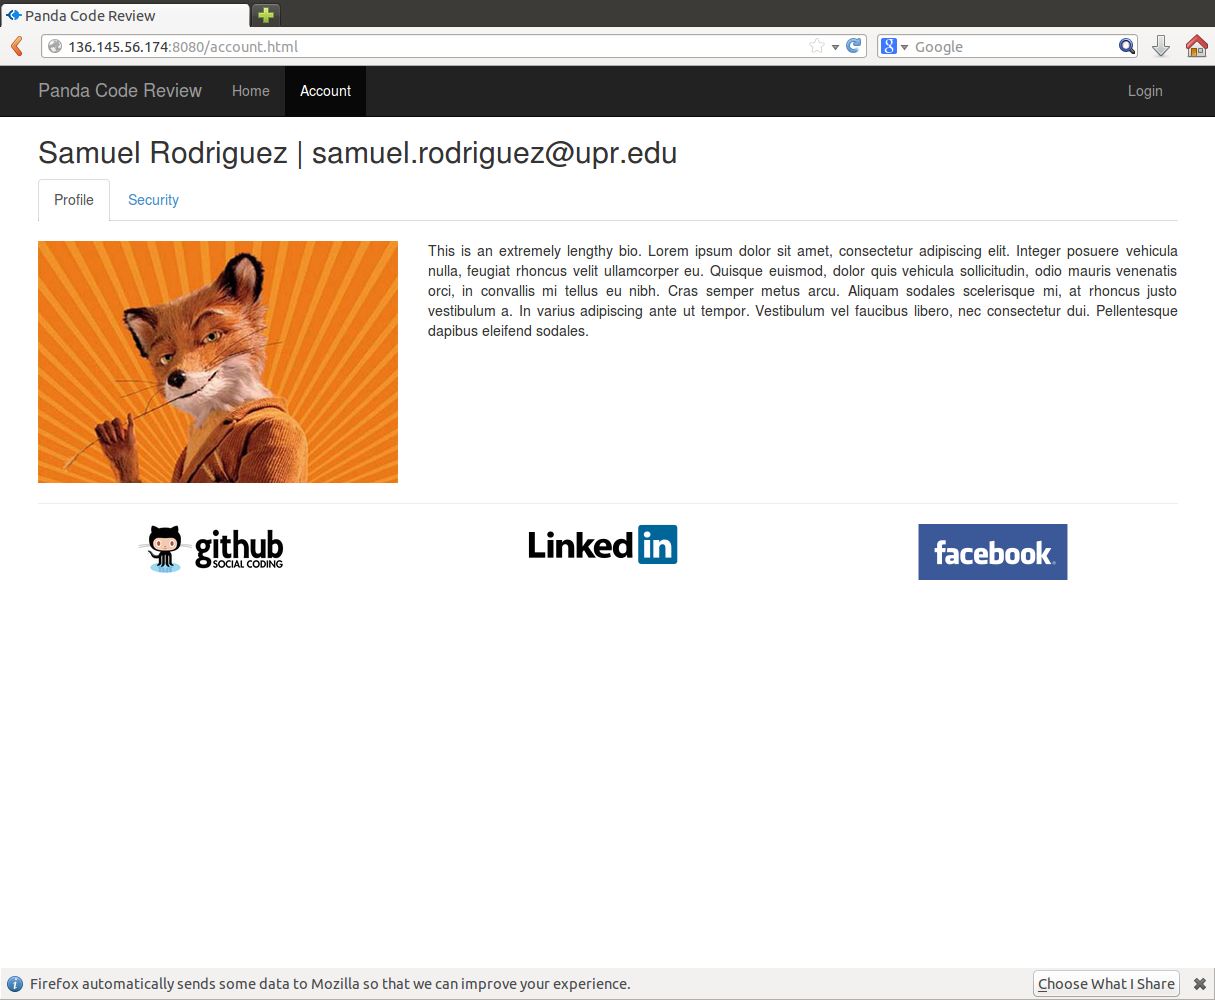
\includegraphics[width=\textwidth]{img/account-profile}
	\caption{Account Profile}
\end{figure}

\textbf{Account Security:} Both students and professors are able to
see their account securities information. This includes the ability to
change their passwords and view, add and remove ssh keys.

\begin{figure}[H]
	\centering
	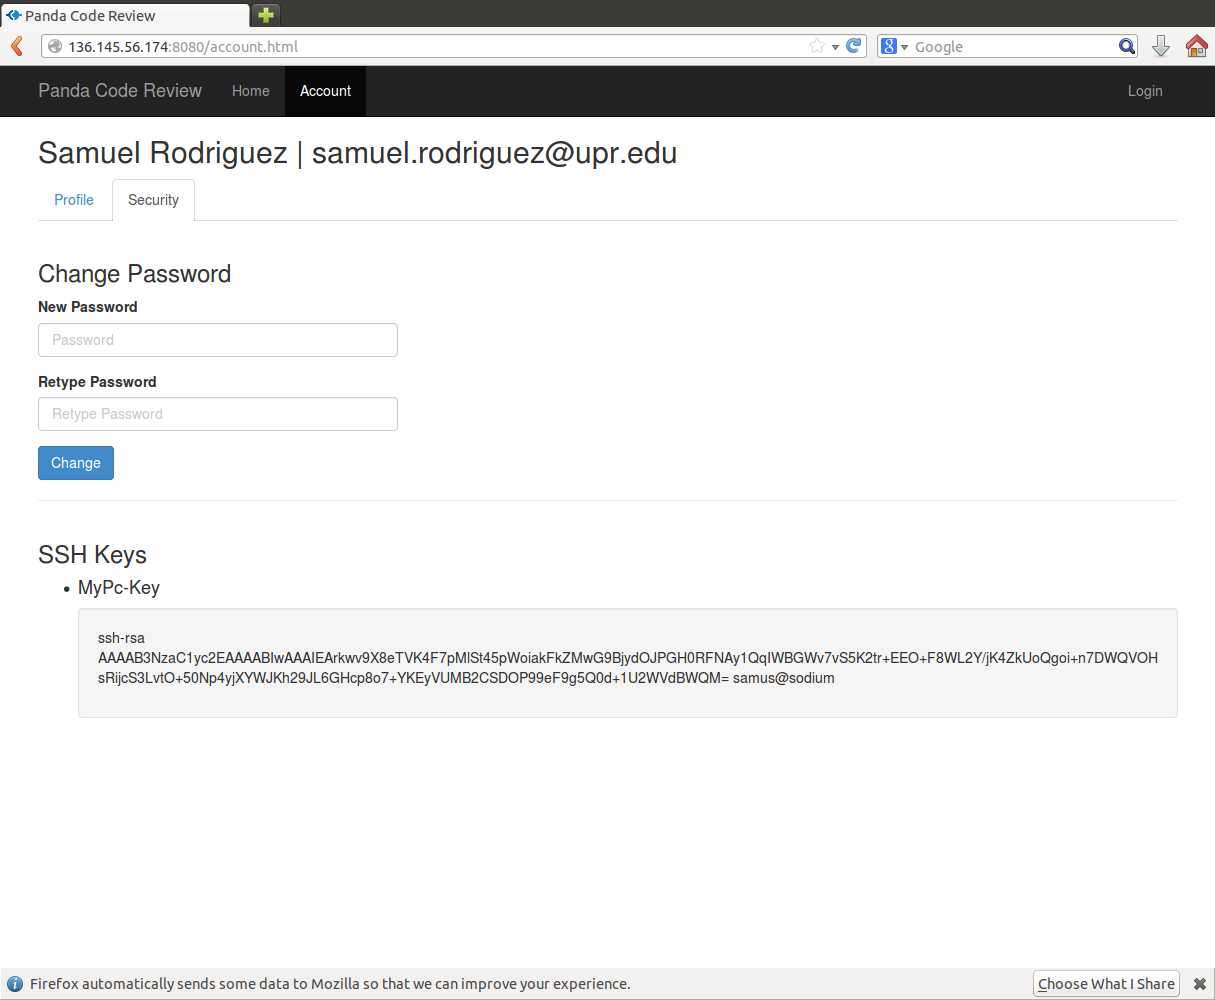
\includegraphics[width=\textwidth]{img/account-secutiry}
	\caption{Account Security}
\end{figure}